\documentclass{article} % For LaTeX2e
\usepackage{nips15submit_e,times}
\usepackage{hyperref}
\usepackage{url}
\usepackage{graphicx}
\usepackage{amsfonts}
\usepackage{amssymb}
\usepackage{float}
\usepackage{listings}
\usepackage{xcolor}
%\documentstyle[nips14submit_09,times,art10]{article} % For LaTeX 2.09


\lstset { %
    language=C++,
    backgroundcolor=\color{black!5}, % set backgroundcolor
    basicstyle=\footnotesize,% basic font setting
}


\title{Problem Set 1 for Machine Learning 15 Fall}


\author{
Jingyuan Liu\\
AndrewId: jingyual\\
\texttt{jingyual@andrew.cmu.edu} \\
}


\newcommand{\fix}{\marginpar{FIX}}
\newcommand{\new}{\marginpar{NEW}}


\nipsfinalcopy % Uncomment for camera-ready version


\begin{document}
\maketitle


\section{Probability and Statistics Review}



\subsection{Exponential Families}
\textbf{(a) Show that Multinomial distribution, Multi-variate Gaussian distribution and
Dirichlet distribution are members of the exponential families.}

\textbf{Multinomial distribution} The probability mass function of multinomial
distribution :

\begin{equation}
\label{equ:multinomial}
f(x_{1},...,x_{k};p_{1},...,p_{k}) = \frac{\Gamma ( \sum_{i} {x_{i}} + 1)}
{\prod_{i} \Gamma (x_{i} + 1)} \cdot \prod_{i}^{K} p_{i}^{x_{i}}
\end{equation}

Here the $x_{i}$ $\in$ X, $p_{i}$ $\in$ $\theta$, and the $\Gamma$ is the Gamma
function:

\begin{equation}
\label{GammaFunction}
\Gamma (n) = (n-1) ! \quad , \qquad \Gamma (t) = \int_0^\infty x^{t-1}e^{-x} dx
\end{equation}

To prove it belongs to exponential families, we can transfer it into:

\begin{equation}
f(X ; \theta) = \frac{\Gamma ( \sum_{i} {x_{i}} + 1)}
{\prod_{i} \Gamma (x_{i} + 1)} \cdot \prod_{i}^{K} p_{i}^{x_{i}}
\end{equation}

\begin{equation}
\qquad \qquad \quad = h(x) \cdot p_1^{x_1} \cdot p_2^{x_2} ... p_i^{x_i} ... p_k^{x_k}
\end{equation}

\begin{equation}
\qquad \qquad \quad = h(x) \cdot exp ( \sum_k x_i \cdot ln(p_i))
\end{equation}

Here $ln(x)$ is $log_e x$. Therefore, we can get

\begin{equation}
h(X)= \frac{\Gamma ( \sum_{i} {x_{i}} + 1)}
{\prod_{i} \Gamma (x_{i} + 1)}
\end{equation}

\begin{equation}
\eta (\theta) = (ln(p_1), ln(p_2),..., ln(p_k))^T
\end{equation}

\begin{equation}
T(X) = (x_1, x_2,..., x_k)^T
\end{equation}

\begin{equation}
A(\theta) = 0
\end{equation}

Simply, we can derive for other specific distributions and prove that they also
belong to exponential families:

\textbf{Gaussian Distribution}, ${ \{ N( \mu, \sigma^2): \mu \in \mathbb{R},
\sigma > 0 \} }$ is:

\begin{equation}
f(X, \theta) = \frac{1}{\sigma \sqrt{2 \pi}} exp(- \frac{(x - \mu)^2}{2 \sigma^2})
\end{equation}

\begin{equation}
\qquad \qquad \qquad \qquad \qquad
= \frac{1}{\sqrt{2 \pi}} exp \{ \frac{\mu}{\sigma^2} x - \frac{1}{2 \sigma^2} x^2 -
\frac{\mu^2}{2 \sigma^2} - ln \sigma\}
\end{equation}

Therefore, we can prove that Gaussian distribution is in exponential families:

\begin{equation}
h(X) = \frac{1}{\sqrt{2 \pi}}
\end{equation}

\begin{equation}
\eta(\theta) = (\frac{\mu}{\sigma^2}, \frac{1}{2 \sigma^2})
\end{equation}

\begin{equation}
T(X) = (x, -x^2)
\end{equation}

\begin{equation}
A(\theta) = \frac{\mu}{2 \sigma^2} + ln \sigma
\end{equation}

\textbf{Gamma Distribution} is:

\begin{equation}
f (X; \theta) = \frac{1}{B( \alpha )} \prod_{i=1}^K x_i^{\alpha_i - 1}
\end{equation}

\begin{equation}
B( \alpha )= \frac{\prod_{i=1}^K \Gamma(\alpha_i)}
{\Gamma (\sum_{i=1}^K \alpha_i)}
\end{equation}

After similar derivation with multinomial, we can get:

\begin{equation}
h(X)  = 1
\end{equation}

\begin{equation}
\eta( \theta ) = (\alpha_1 - 1, \alpha_2 - 1, ..., \alpha_i - 1, ..., \alpha_k -
1)^T
\end{equation}

\begin{equation}
T(X)  = (ln(x_1), ln(x_2), ..., ln(x_i), ..., ln(x_k))^T
\end{equation}

\begin{equation}
A(\theta) = - ln(B(\alpha))
\end{equation}


\textbf{(b) Computer the posterior}

Based on Bayes Rule, we know that:

\begin{equation}
p(\theta \mid x)  = \frac{p(x \mid \theta) \cdot p(\theta)}{p(x)}
\end{equation}

The $p(\theta \mid x)$ is the posterior, the $p(x \mid \theta)$ is the likelihood,
the $p(\theta)$ is the prior, and the $p(x)$ is the evidence. Given dataset
$D = \{ x_i \}_{i=1}^N$, the evidence is observed, so we can get:

\begin{equation}
p(\mathcal{X, V} \mid X) \propto p(X \mid \theta) \cdot p(\theta \mid
\mathcal{X, V})
\end{equation}

And the observed data is supposed to be iid., therefore, the likelihood :

\begin{equation}
p(X \mid \theta) = \prod_{i=1}^N p(x_i) = \prod_{i=1}^N h(x_i) exp( \theta^T
T(x_i) - A(\theta))
\end{equation}

Therefore, the posterior is in the form of :
\begin{equation}
p(\mathcal{X, V} \mid X) \propto
\prod_{i=1}^N h(x_i) exp( \theta^T T(x_i) - A(\theta))
\cdot f(\mathcal{X, V}) exp({\theta^T \mathcal{X} - \mathcal{V}A(\theta)})
\end{equation}

\begin{equation}
\qquad \qquad \qquad = \prod_{i=1}^N h(x_i) \cdot f(\mathcal{X, V}) \cdot
exp(\theta^T (\sum_{i=1}^N T(x_i) + \mathcal{X}) - (N + \mathcal{V}) A(\theta))
\end{equation}

Therefore, we can see that the posterior takes the same form as the prior.


\subsection{Maximum Likelihood Estimation}
\textbf{a. Prove $A'(\hat\theta_{ML}) = \frac{1}{N}\sum\limits_i T(X_i)$}

Given tge datasets, we can get the log likelihood function:

\begin{equation}
log(p(X)) = \prod_{i=1}^N log(p(x_i))
= \sum_{i=1}^N log(h(x_i)) + \theta \sum_{i=1}^N x_i - N A(\theta)
\end{equation}

We want to maximize the likelihood, which is the same as log likelihood
function considering that log is a convex function, therefore we can get :

\begin{equation}
\frac{\partial log(p(x))}{\partial \theta} = \sum_{i=1}^N T(x_i) - N A'(\theta)
\end{equation}

Then at the maximal point, the partial would be 0, so we can prove it:

\begin{equation}
A'(\hat\theta_{ML}) = \frac{1}{N}\sum\limits_i T(X_i)
\end{equation}


\textbf{b. Compute the uniform distribution maximal likelihood}

As we can see from the uniform distribution, we can get the log likelihood :

\begin{equation}
log(p(x \mid \theta)) = \sum_{i=1}^{N} log(\frac{1}{\theta})
\end{equation}

Therefore, to maximize the log likelihood, we can get the partial descent :

\begin{equation}
\frac{\partial log(p(x \mid \theta))}{\partial \theta}
= - \sum_{x=1}^{N} \theta^{-1} = - \frac{N}{\theta} < 0
\end{equation}

We can see that the likelihood is decreasing with the increase of
$\theta$. So when the $\theta$ get the minimual value, the likelihood can get
the max value. Therefore, $\theta_{ML}$ should be $\frac{1}{x_{max}}$.



\section{Decision Boundary of Naive Bayes}

\subsection{Compute posterior and decision boundary}
The posterior for $p(Y=1 \mid X)$ is :

\begin{equation}
p(Y=1 \mid X) = \frac{p(X \mid Y=1) \cdot p(Y=1)}{p(X)}
\end{equation}

\begin{equation}
\qquad \qquad = \frac{\prod_{i=1}^d p(X_i \mid Y=1) \cdot p(Y=1)}
{\sum_y \prod_{i=1}^d p(X_i \mid Y) \cdot p(Y)}
\end{equation}

\begin{equation}
= \frac{\prod_i^d h(x_i) exp(\theta_{i1} T_i(x_i) - A_i(\theta_{i1})) \pi}
{\prod_i^d h(x_i) (exp(\theta_{i1} T_i(x_i) - A_i(\theta_{i1})) \pi +
exp(\theta_{i0} T(x_i) - A_i(\theta_{i0})) (1 - \pi))}
\end{equation}

\begin{equation}
= \prod_i^d \frac{1}
{1 + (\frac{1 - \pi}{\pi}) exp(T(x_i)(\theta_{i0} - \theta_{i1}) -
(A_i(\theta_{i0}) - A_i(\theta_{i1})))}
\end{equation}

\begin{equation}
= \prod_i^d \sigma((\theta_{i0 - \theta_{i1}})T(X_i) - (A_i(\theta_{i0}) -
A_i(\theta_{i1})) - k)
\end{equation}

Here, k is:
\begin{equation}
k = exp(ln(\frac{1-\pi}{\pi}))
\end{equation}

And posterior for $p(Y=1 \mid X)$ is similar to this. To compute the decision
boundary, we do not need to care the denominer, considering that given a
observed dataset, the $p(x)$ remains the same. So we can get:

\begin{equation}
P(X \mid Y= 1) \cdot p(Y=1) = P(X \mid Y = 0) \cdot p(Y=0)
\end{equation}

\begin{equation}
log (\prod_i h(x_i) exp(\theta_{i1} T(x_i) - A_i(\theta_{i1})) \pi)
= log (\prod_i h(x_i) exp(\theta_{i0} T(x_i) - A_i(\theta_{i0}) (1- \pi)))
\end{equation}

\begin{equation}
\label{decision}
\sum_i \theta_{i1} T_{i1}(x_i) - A_i(\theta_{i1}) + log(\pi) =
\sum_i \theta_{i0} T_{i0}(x_i) - A_i(\theta_{i0}) + log(1 - \pi)
\end{equation}

For those x which satisfy the equation \ref{decision}, we would get the decision
boundary.


\subsection{Gaussian linear boundary}

As the equation (\ref{decision}) shows, and that $P(X_i \mid Y)$ is a Gaussian
Distribution, we could get:

\begin{equation}
\sum_i \frac{\mu_{i1}}{\sigma_{i1}^2} x - \frac{1}{2 \sigma_{i1}^2} x^2 - k_{i1} =
\sum_i \frac{\mu_{i0}}{\sigma_{i0}^2} x - \frac{1}{2 \sigma_{i0}^2} x^2 - k_{i0}
\end{equation}

Here k is constants changing with i, but is not related to x or parameters.
Considering that $\sigma$ is not related with label, we can get:

\begin{equation}
\sum_i \frac{\mu_{i1}}{\sigma_{i1}^2} x - k_{i1} =
\sum_i \frac{\mu_{i0}}{\sigma_{i0}^2} x - k_{i0}
\end{equation}

Therefore, we could get that the decision boundary is linear in terms of X.



\section{KNN Classification}


\subsection{Question (a)}
I think it is impossiable to build a decision tree as descripted that exactly behave
the same as the 1-NN classifier.

As the following figure \ref{fig:knn} shows, we could see 1-NN would split the
region into several parts, and in different parts, the classification result is
different.While for decision tree, it could only split the area horizontly or
vertically. Therefore, the classifiers based on these two models migh not behave
exactly the same. 

\begin{figure}[!htbp]
\begin{center}
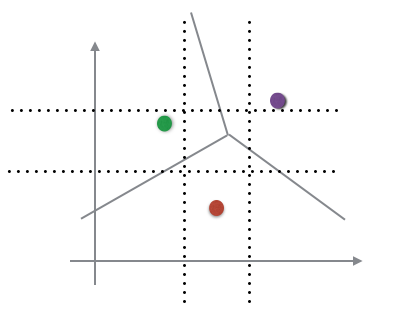
\includegraphics[width=60mm]{pic/knn.png}
\end{center}
\label{fig:knn}
\caption{1-NN Classifier vs ``Binary'' Decision Tree}
\end{figure}


\subsection{Question (b)}
We could set a special example to explain. Suppose we have only one dimension
continuous variable and two points, with $x_0$ = 0, $x_1$ = 1. And we choose k = 2.

Then, we use the model to do classification. Suppose we have a new x, it could
fall into three areas. We could notice that, when x falls between $x_0$ and
$x_1$, the probabilty is $\frac{K}{NV} \cdot v'$, which equals 1. Then we could
also find that the probability that x falls before $x_0$ and after $x_1$ is also
positive, therefore, the overall probability is bigger than 1, which is
unreasonable.


\subsection{Question (c)}
Considering that $p(e \mid x)$ is the limit that N is going to limit, so we
could see here, x' is x in the limited case. Therefore, we could deriviate:

\begin{equation}
p_N(e \mid x) - p(e \mid x) =
p(c_1 \mid x) p(c_2 \mid x') + p(c_2 \mid x) p(c_1 \mid x')
- p(c_1 \mid x) p(c_2 \mid x ) + p(c_2 \mid x) p(c_1 \mid x)
\end{equation}

\begin{equation}
= p(c_1 \mid x) (p(c_2 \mid x') - p(c_2 \mid x))
+ p(c_2 \mid x) (p(c_1 \mid x') - p(p_1 \mid x))
\end{equation}

If we use the distance as describe in the note, then we could get:

\begin{equation}
p_N(e \mid x) - p(e \mid x)
= a (d_{c2}(x, x'))
+ (1-a) {d_{c1}(x,x')}
\end{equation}

Where $a = p(c_1 \mid x)$. $d_{c2}(x, x') = -d_{c1}(x,x')$, because
$p(c_2 \mid x) + p(c_1 \mid x) = 1$. So :

\begin{equation}
E((p_N - p)^2 \mid x) = (d(x,x') -2ad(x,x'))^2
\end{equation}

Therefore, in this case, we would have the minimal value for the upperbound.



\section{Decision Trees}


\subsection{Decision tree on two features}
\textbf{Question (a)}

Removing x' from the trainning dataset would change the learnt decision tree. I
think there would be two main reasons:

(1) First, removing a ``column'' from dataset would change the conditional
probability $p(X \mid Y)$, so it might influence the information gain for a certain
feature, and influence us on choosing the best feature to split.

(2) Second, it would also influence us to decide the split result on a label.
Removing x' from dataset may influence us that which is the majority case after
splitting the feature.

\textbf{Question (b) and Question (c)}
I think that in both the (b) and (c) case, the decision tree could correctly
classify these vectors. The upper bound for both case is $log_2^n$, where n is
the total number of the data points. My method to prove it is the same for both
cases.

Let's use figures to show the meaning of it. If we have a total number of N
points, and we want fit all data point. Given our classification tree model, we
could see that each time we build one more layer, then we could split the total
region into two times subregions. So in total, if we have K layers, then we
could split the region into $2^k$ subregions.

\begin{figure}[!htbp]
\begin{center}
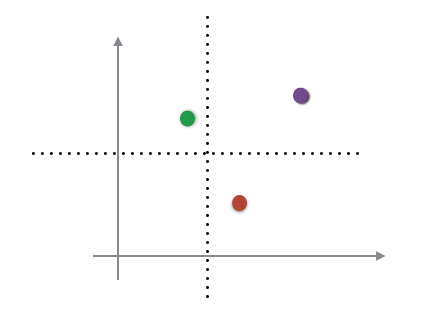
\includegraphics[width=60mm]{pic/k2dt.png}
\end{center}
\label{fig:k2dt}
\caption{k = 2, 4 splitted subregions}
\end{figure}

\begin{figure}[!htbp]
\begin{center}
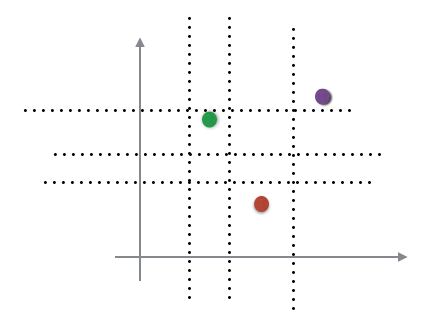
\includegraphics[width=60mm]{pic/k4dt.png}
\end{center}
\label{fig:k4dt}
\caption{k = 4, 16 splitted subregions}
\end{figure}

Therefore, for N points and k layers, we could always build $2^k$ subregions.
The upper bound is that N points falls into each subregions, so we need to
assign each subregion a different label. Therefore:

\begin{equation}
2^k = N \qquad \qquad  k = log_2(N)
\end{equation}


\subsection{C4.5 Algorithm}
I implemented ID3 and C4.5 Decision tree via Weka Interface, which is a data
mining software. The ID3 tree was in Weka but not suitable to do the
classification and I exported the trainning output. The C4.5 was J48 in Weka
library.  The two trees are as follows:

\begin{figure}[!htbp]
\begin{center}
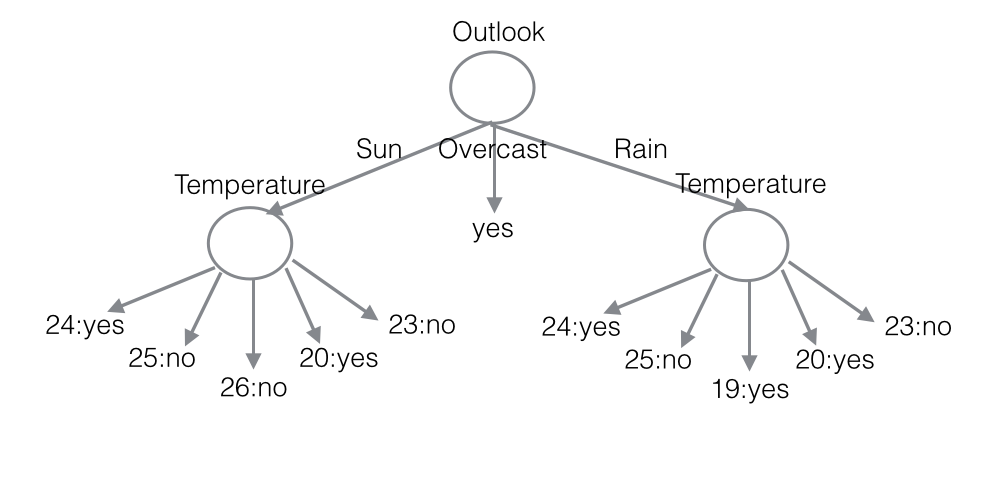
\includegraphics[width=120mm]{pic/id3.png}
\end{center}
\label{id3}
\caption{ID3 Decision Tree}
\end{figure}

\begin{figure}[!htbp]
\begin{center}
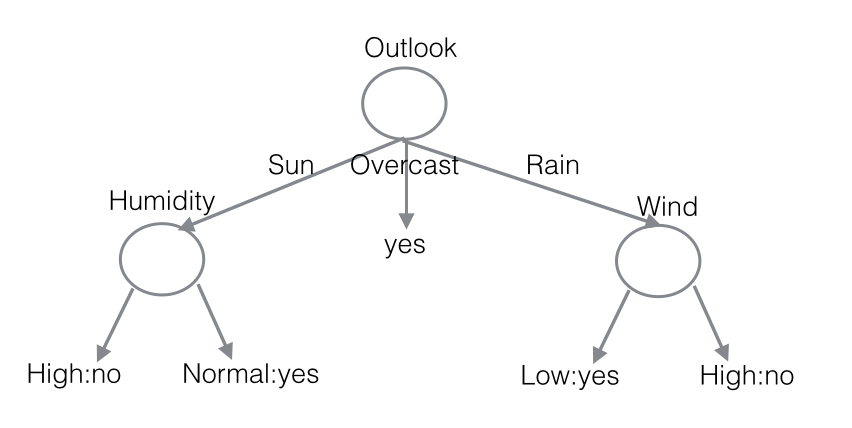
\includegraphics[width=120mm]{pic/c45.png}
\end{center}
\label{c45}
\caption{C4.5 Decision Tree}
\end{figure}

As we can see from these two figures, the ID3 prefer the features with larger V,
like temperature, while C4.5 prefer the features with smaller V.



\section{Naive Bayes}


\subsection{Result Analysis}
I implemented Naive Bayes using C++. It costs more time than I planned...
Feeling sad, I only finished the task one, preprocessment and classification.
I did not do experiment with code. Next time, I would choose python or
allocate more time for c++.

The result :

(1) For Train Datasets:

Neg Precision: 0.98375, Pos Precision: 0.9475, Overall Precision: 0.967125

(2) For Test Datasets:

Neg Precision: 0.34, Pos Precision: 0.28, Overall Precision: 0.31

As we can see, the trainning precision is fairly high while the testing
precision is very low. The implemented model should be overfitted.


\subsection{Running code}
I design a Data class to preprocess data, a Model class to train the model, and
the Evaluation clas to evaluate the result. To run the code, you would need to
change the rootPaht in the data.cc to your local file path to load data from
your disk. After this change, type make and run the ./main, it will run the
overall program and then output the neg precision and pos precision seperately.



\section{Collaboration}
I discussed with Zheng Chen from MIIS Program with Question 3 and Question 4.
Specifically, we discussed how to understand the layer relationship with the
splitted subregions. Therefore we could solve Question 3.a, 4.1.b, and 4.1.c.



\section{Code}

(1) Makefile

\lstinputlisting[language=C++]{CMakefile}


(2) Data class

\lstinputlisting[language=C++]{data.h}
\lstinputlisting[language=C++]{data.cc}


(3) Model class

\lstinputlisting[language=C++]{model.h}
\lstinputlisting[language=C++]{model.cc}

(4) Evaluation class

\lstinputlisting[language=C++]{evaluation.h}
\lstinputlisting[language=C++]{evaluation.cc}

(5) Main

\lstinputlisting[language=C++]{main.cc}


\end{document}
